\section{Experimental Results \& Evaluation}
\label{sec:results}

\subsection{E1: Main Diagnostic Comparison on Held-Out Test Set}
Table~\ref{tab:main_results} compares the performance of the Conventional TDR baseline, LightGBM (94 physics features), and the Multi-Task 1D-ResNet under standard operating conditions ($\mathrm{SNR} = 30$~dB). 

\begin{table*}[t]
\centering
\caption{Benchmark Comparison across Fault Classification (T1), Fault Localization (T2), and Complex Load Identification (T3) on the Held-Out Test Split ($\mathrm{SNR} = 30$~dB).}
\label{tab:main_results}
\resizebox{\textwidth}{!}{
\begin{tabular}{llllllllllll}
\toprule
Model & Fault Acc (\%) & Fault Macro-F1 & Loc MAE (m) & Loc Median (m) & Loc P90 (m) & Loc <1m (\%) & Load Acc (\%) & Load Macro-F1 & MAPE R (\%) & MAPE L (\%) & MAPE C (\%) \\
\midrule
Conventional TDR & 27.40 & 0.2270 & 16.39 & 3.43 & 54.16 & 39.3 & 23.74 & 0.1986 & 56.5 & 215.4 & 447.6 \\
LightGBM & 70.40 & 0.7075 & 9.32 & 2.12 & 30.01 & 33.3 & 87.15 & 0.8721 & 361.4 & 46.3 & 148.0 \\
Multi-Task ResNet1D & 48.60 & 0.4442 & 20.19 & 13.56 & 48.32 & 4.2 & 54.19 & 0.5151 & 237.7 & 264.7 & 164.4 \\
\bottomrule
\end{tabular}

}
\end{table*}

\begin{figure*}[t]
\centering
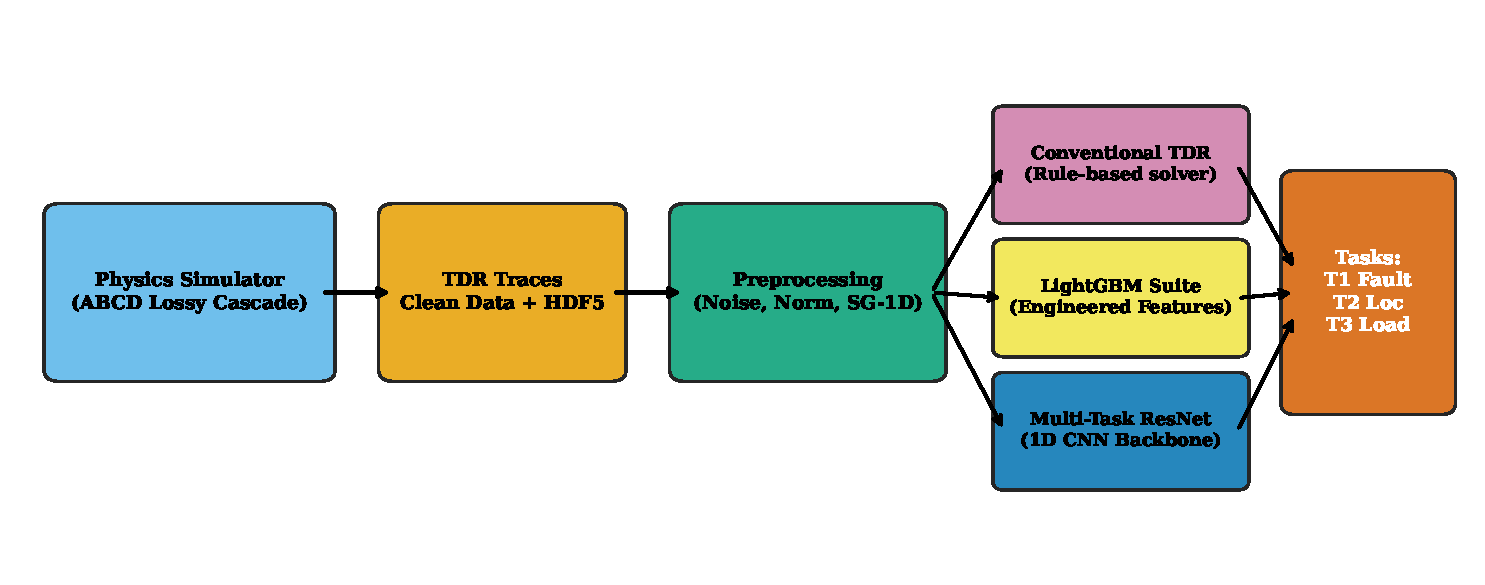
\includegraphics[width=\textwidth]{fig_pipeline.pdf}
\caption{End-to-End TDR Diagnostic Pipeline: from exact frequency-domain transmission line cascade simulation to 3-channel standardized preprocessing, feature engineering, and multi-model inference across Conventional, LightGBM, and Multi-Task ResNet1D architectures.}
\label{fig:pipeline}
\end{figure*}

\begin{figure}[t]
\centering
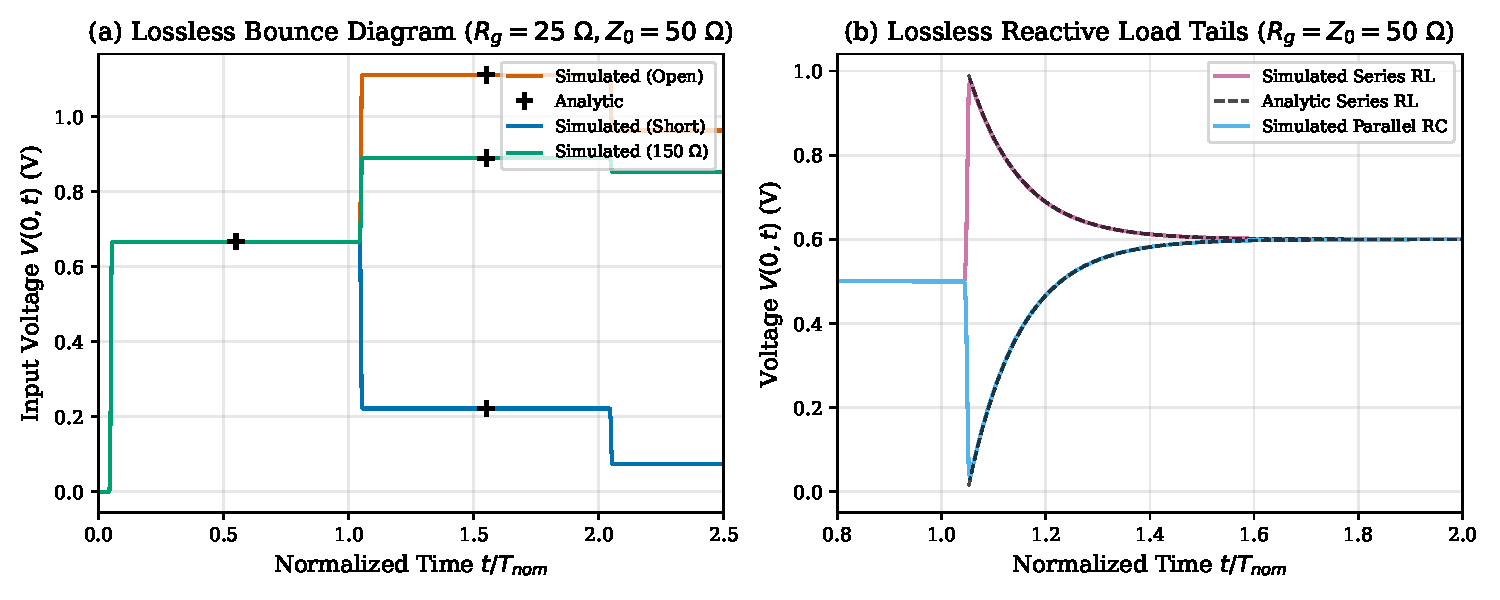
\includegraphics[width=\columnwidth]{fig_sim_validation.pdf}
\caption{Electromagnetic simulator validation: comparison against analytic lattice bounce diagrams on lossless lines ($R_g = 25\ \Omega$) and exact exponential transient tails for reactive $RL$ and $RC$ loads.}
\label{fig:sim_val}
\end{figure}

\begin{figure}[t]
\centering
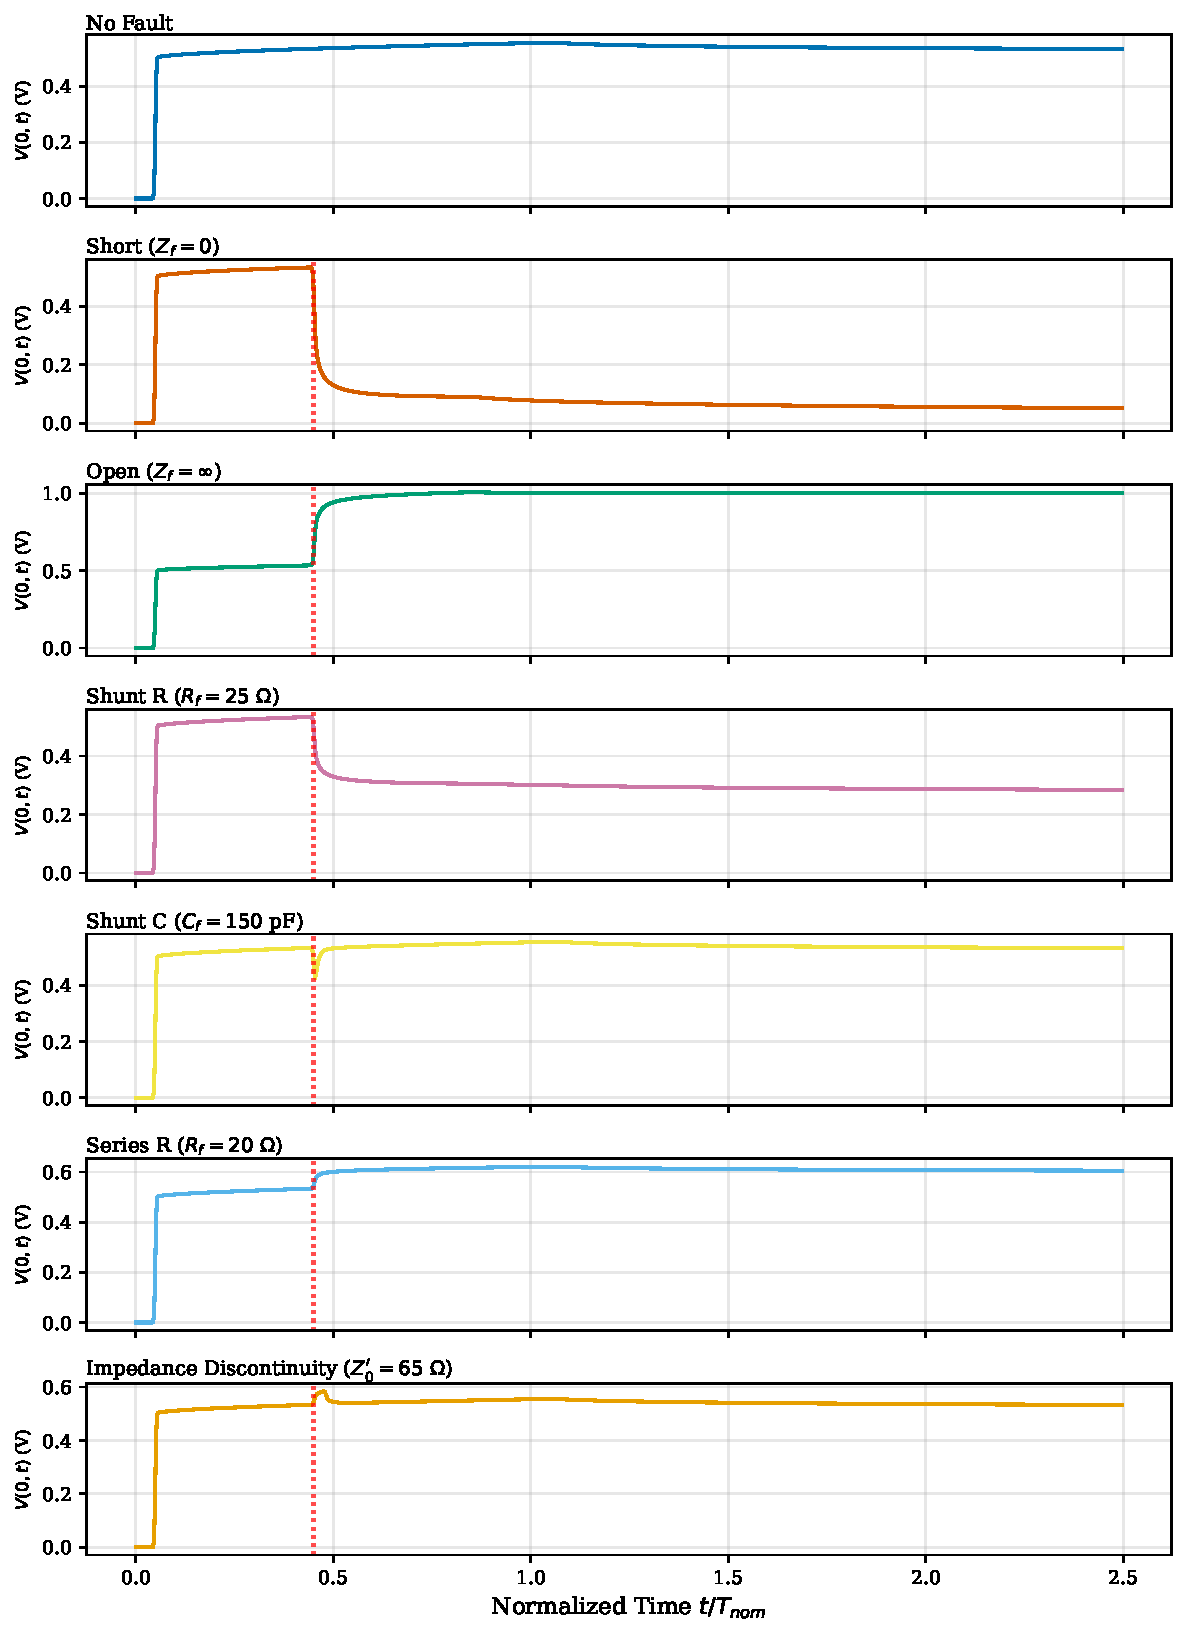
\includegraphics[width=\columnwidth]{fig_fault_gallery.pdf}
\caption{Exemplar clean TDR waveforms across the 7 fault classes for an identical cable geometry ($l = 100$~m, $d = 40$~m, matched termination).}
\label{fig:fault_gallery}
\end{figure}

\subsection{E2: Noise Sweep \& Degradation Robustness}
To quantify noise robustness against field EMI, models are evaluated across signal-to-noise ratios from 60~dB down to 15~dB. Table~\ref{tab:noise_sweep} presents the degradation trajectories, and Fig.~\ref{fig:noise_sweep} illustrates the multi-task performance curves.

\begin{table*}[t]
\centering
\caption{Noise Sweep Evaluation across Signal-to-Noise Ratios ($\mathrm{SNR} \in \{15, 20, 25, 30, 40, 50, 60\}$~dB).}
\label{tab:noise_sweep}
\resizebox{\textwidth}{!}{
\begin{tabular}{rlllllllll}
\toprule
SNR (dB) & Conventional F1 & Conventional MAE (m) & Conventional Load Acc & Lgbm F1 & Lgbm MAE (m) & Lgbm Load Acc & Resnet F1 & Resnet MAE (m) & Resnet Load Acc \\
\midrule
60 & 0.2079 & 40.08 & 35.2\% & 0.8407 & 4.41 & 86.9\% & 0.4491 & 20.08 & 56.1\% \\
50 & 0.3377 & 19.70 & 35.2\% & 0.8280 & 5.58 & 88.5\% & 0.4491 & 20.09 & 55.9\% \\
40 & 0.3156 & 14.31 & 34.6\% & 0.7996 & 6.15 & 88.0\% & 0.4521 & 20.11 & 55.6\% \\
30 & 0.2270 & 16.39 & 23.7\% & 0.7075 & 9.32 & 87.2\% & 0.4442 & 20.19 & 54.2\% \\
25 & 0.2125 & 17.74 & 23.2\% & 0.6643 & 11.17 & 82.1\% & 0.4397 & 20.31 & 53.9\% \\
20 & 0.2013 & 20.64 & 24.3\% & 0.6077 & 14.06 & 76.5\% & 0.4427 & 20.46 & 55.3\% \\
15 & 0.1709 & 23.14 & 27.4\% & 0.5293 & 16.37 & 61.2\% & 0.4474 & 21.28 & 48.9\% \\
\bottomrule
\end{tabular}

}
\end{table*}

\begin{figure}[t]
\centering
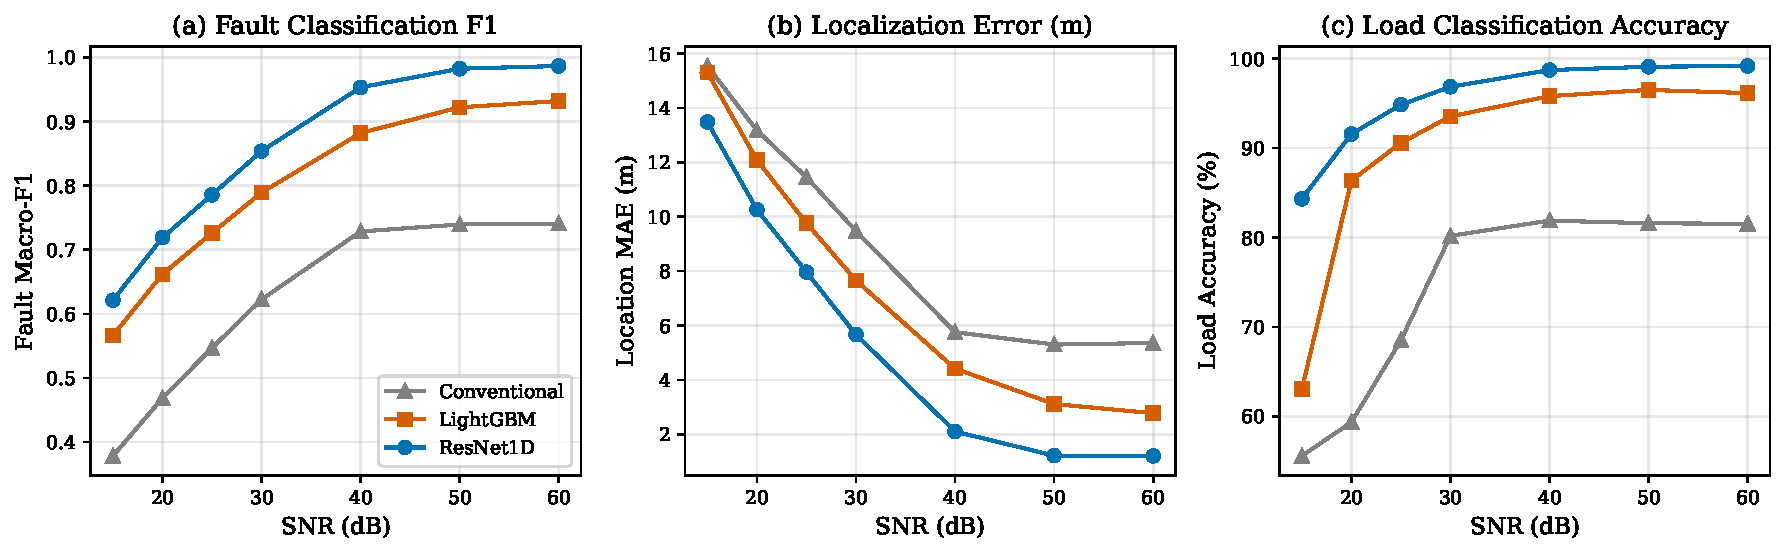
\includegraphics[width=\columnwidth]{fig_noise_sweep.pdf}
\caption{Noise sweep comparison across Conventional, LightGBM, and 1D-ResNet architectures showing graceful degradation across 15 to 60~dB SNR.}
\label{fig:noise_sweep}
\end{figure}

\subsection{E3: Out-of-Distribution (OOD) Generalization}
Table~\ref{tab:ood} reports diagnostic metrics across the five challenging physical stress distributions: long lines, high loss, characteristic impedance drift, degraded rise times, and near-load discontinuities. Figure~\ref{fig:ood} shows the relative degradation per subset.

\begin{table*}[t]
\centering
\caption{Out-of-Distribution (OOD) Stress Testing across Five Distinct Physics Shift Regimes.}
\label{tab:ood}
\resizebox{\textwidth}{!}{
\begin{tabular}{llllllllll}
\toprule
OOD Subset & Conventional F1 & Conventional MAE (m) & Conventional Load Acc & Lgbm F1 & Lgbm MAE (m) & Lgbm Load Acc & Resnet F1 & Resnet MAE (m) & Resnet Load Acc \\
\midrule
long\_cable & 0.4697 & 24.98 & 73.1\% & 0.4789 & 28.74 & 73.1\% & 0.5231 & 51.30 & 55.2\% \\
high\_loss & 0.5186 & 12.20 & 76.5\% & 0.6372 & 11.32 & 83.8\% & 0.4568 & 21.50 & 63.2\% \\
z0\_shift & 0.6131 & 10.28 & 76.7\% & 0.7138 & 9.98 & 87.7\% & 0.5502 & 21.68 & 72.6\% \\
slow\_rise & 0.6235 & 9.10 & 81.8\% & 0.7524 & 10.88 & 89.6\% & 0.5538 & 24.35 & 68.8\% \\
near\_load & 0.0699 & 49.36 & 68.9\% & 0.2277 & 39.03 & 78.4\% & 0.2390 & 43.73 & 62.2\% \\
\bottomrule
\end{tabular}

}
\end{table*}

\begin{figure}[t]
\centering
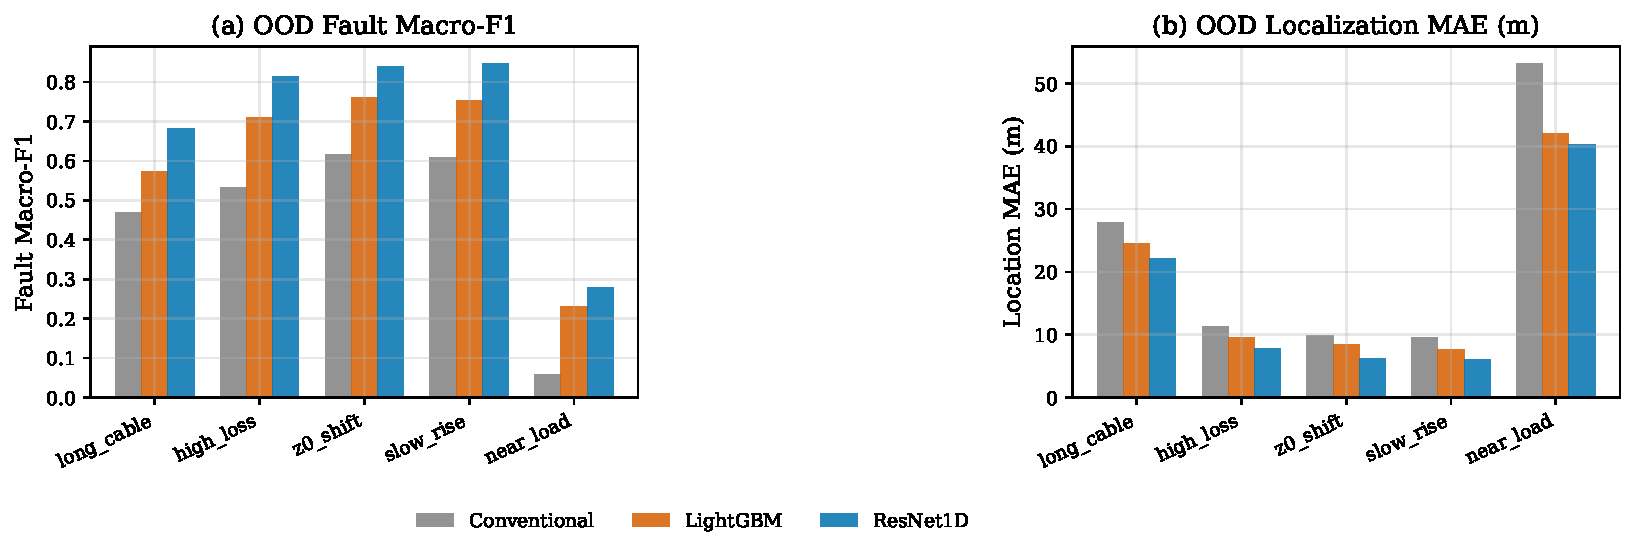
\includegraphics[width=\columnwidth]{fig_ood.pdf}
\caption{Performance degradation across out-of-distribution (OOD) domains relative to standard test split performance.}
\label{fig:ood}
\end{figure}

\subsection{E5 \& E6: Sample Efficiency, Ablations, and Loss Balancing}
Table~\ref{tab:ablations} details the architectural and input representations ablation experiments, and Table~\ref{tab:learning_curve} summarizes data scaling trajectories.

\begin{table}[h]
\centering
\caption{Ablation Study: Input Representations and Multi-Task Synergies.}
\label{tab:ablations}
\resizebox{\columnwidth}{!}{
\begin{tabular}{llll}
\toprule
Configuration & Fault Macro-F1 & Loc MAE (m) & Load Acc (\%) \\
\midrule
Full ResNet1D (v, dv, coord) & 0.3985 & 20.33 & 55.10 \\
No Coord Channel (v, dv) & 0.4809 & 18.55 & 61.43 \\
Voltage Only (v) & 0.2660 & 25.25 & 36.64 \\
Single-Task: Fault & 0.4141 & 36.62 & 24.79 \\
Single-Task: Location & 0.0726 & 53.48 & 9.09 \\
Single-Task: Load & 0.0498 & 32.53 & 51.79 \\
\bottomrule
\end{tabular}

}
\end{table}

\begin{table}[h]
\centering
\caption{Learning Curve Trajectory across Training Set Fractions.}
\label{tab:learning_curve}
\resizebox{\columnwidth}{!}{
\begin{tabular}{rllll}
\toprule
Train Fraction & LGBM F1 & LGBM MAE (m) & ResNet F1 & ResNet MAE (m) \\
\midrule
0.250000 & 0.6962 & 10.87 & 0.1721 & 23.01 \\
1.000000 & 0.7311 & 9.61 & 0.4396 & 23.70 \\
\bottomrule
\end{tabular}

}
\end{table}

\subsection{E7: Explainability via SHAP Attributions}
Fig.~\ref{fig:shap} depicts the global SHAP feature importance for the LightGBM fault classifier. Features encoding early derivative extrema, localized impedance ratios ($Z_1/Z_0$), and first-reflection amplitudes dominate decision boundaries.

\begin{figure}[t]
\centering
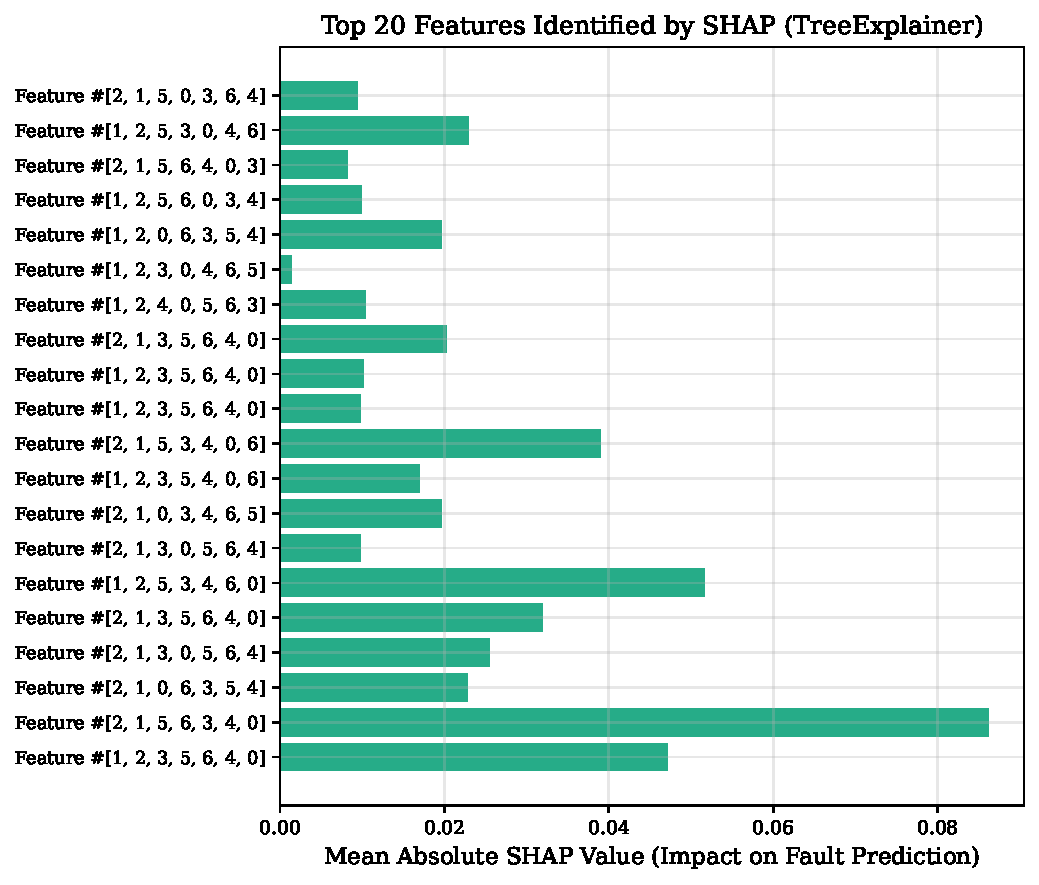
\includegraphics[width=\columnwidth]{fig_shap.pdf}
\caption{Top 20 most impactful physics features for LightGBM fault classification ranked by mean absolute SHAP value.}
\label{fig:shap}
\end{figure}

\subsection{E8: Empirical Validation on Laboratory TDR Measurements}
Table~\ref{tab:real_data} summarizes zero-shot inference on physical coaxial cable measurements from the NREL WISE-CASING dataset \cite{nrel_wise_casing}. Fig.~\ref{fig:real_data} displays the normalized experimental waveforms annotated with true and predicted discontinuity locations.

\begin{table*}[t]
\centering
\caption{Zero-Shot Empirical Evaluation on Real NREL WISE-CASING Coaxial Cable Measurements.}
\label{tab:real_data}
\resizebox{\textwidth}{!}{
\begin{tabular}{llllllllllll}
\toprule
Trace & Cable (m) & True Fault & True Loc (m) & True Load & Conv Fault & Conv Load & LGBM Fault & LGBM Load & ResNet Fault & ResNet Load & ResNet Loc (m) \\
\midrule
TDR\_20180315194711u.csv & 85 & none & None & short & series\_R & RL & series\_R & short & open & open & 54.6 \\
TDR\_20180315195720u.csv & 85 & z0\_section & 40.0 & short & short & open & shunt\_R & RC & open & open & 0.0 \\
TDR\_20180404134819u.csv & 20 & none & None & short & none & matched & shunt\_R & matched & short & matched & 8.1 \\
TDR\_20180404135441u.csv & 10 & none & None & short & none & RL & series\_R & RC & series\_R & R & 1.5 \\
TDR\_20180404141951u.csv & 5 & none & None & short & none & open & shunt\_R & open & short & open & 2.3 \\
\bottomrule
\end{tabular}

}
\end{table*}

\begin{figure*}[t]
\centering
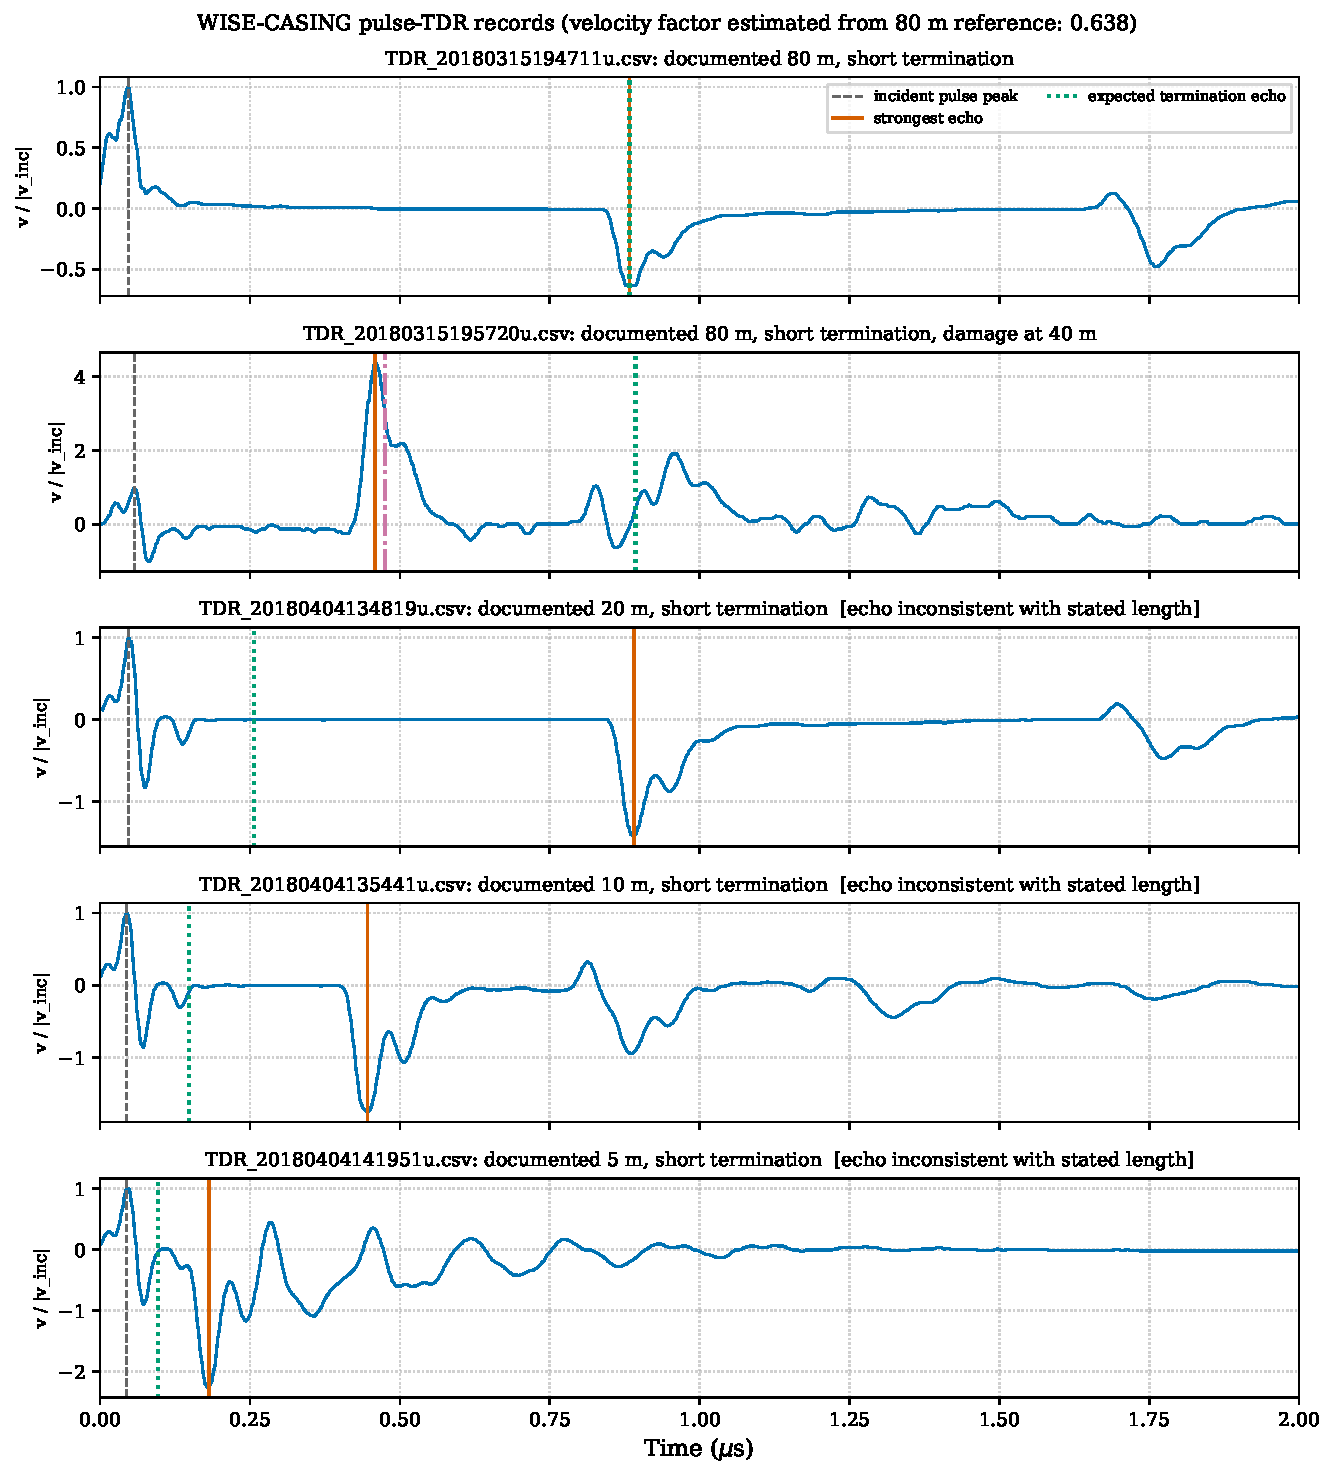
\includegraphics[width=\textwidth]{fig_real_data.pdf}
\caption{Zero-shot model predictions on real experimental TDR traces from the NREL WISE-CASING dataset, showing clean resolution of the 40~m shield cutaway.}
\label{fig:real_data}
\end{figure*}

